\documentclass[aspectratio=169]{beamer}
\usetheme{simple}

\RequirePackage[l2tabu, orthodox]{nag}


% \usepackage[left=1.in, right=1.in, top=1.25in, bottom=1.25in]{geometry}

% FONTS
%\usepackage[T1]{fontenc}

% Replace default Latin Modern typewriter with its proportional counterpart
% http://www.tug.dk/FontCatalogue/lmoderntypewriterprop/
%\renewcommand*\ttdefault{lmvtt}


%%% OPTION 1 - Fourier Math + New Century Schoolbook + ParaType Sans

% % Import Fourier Math (this imposes its own New Century Schoolbook type)
% % http://www.ctan.org/tex-archive/fonts/fouriernc/
%\usepackage{fouriernc}
%\usepackage{amsmath}
% % Replace with TeX Gyre Schola version of New Century Schoolbook (must scale!)
% % http://www.tug.dk/FontCatalogue/tgschola/
%\usepackage[scale=0.92]{tgschola}
%\usepackage[scaled=0.88]{PTSans}

%% OPTION 2 - MathDesign Math + Bitstream Charter + ParaType Sans

% Import MathDesign (this brings along Bitstream Charter)
% http://www.ctan.org/tex-archive/fonts/mathdesign/
\usepackage[bitstream-charter]{mathdesign}
\usepackage{amsmath}
\usepackage[scaled=0.92]{PTSans}


% %%% OPTION 3 - MTPRO 2 Math + Termes Times + ParaType Sans

% \usepackage{tgtermes}
% \usepackage{amsmath}
% \usepackage[subscriptcorrection,
%             amssymbols,
%             mtpbb,
%             mtpcal,
%             nofontinfo  % suppresses all warnings
%            ]{mtpro2}
% \usepackage{scalefnt,letltxmacro}
% \LetLtxMacro{\oldtextsc}{\textsc}
% \renewcommand{\textsc}[1]{\oldtextsc{\scalefont{1.10}#1}}
% \usepackage[scaled=0.92]{PTSans}

% Use default fonts here
\usepackage{amsmath}
\usepackage{amssymb}

% \usepackage{titling}

% % COLOR
% \usepackage[table,usenames,dvipsnames]{xcolor}
\definecolor{shadecolor}{gray}{0.9}

% SPACING and TEXT
\usepackage[final,expansion=alltext]{microtype}
\usepackage[english]{babel}
\usepackage[parfill]{parskip}
\usepackage{afterpage}
\usepackage{framed}
\usepackage{verbatim}
\usepackage{setspace}

\newenvironment{exercise}[1]
{
    \itshape
    \paragraph{Exercise: \textit{#1}}
}
{ 
}


% \usepackage[bottom]{footmisc}
\usepackage[symbol]{footmisc}
\renewcommand{\thefootnote}{\arabic{footnote}}


% FIGURES
\usepackage{graphicx}
\usepackage[labelfont={it, small}, 
            textfont={small,singlespacing},
            % justification={justified,RaggedRight},
            singlelinecheck=false,
            margin=0pt]{caption}
\usepackage[format=hang]{subcaption}
% \usepackage{ccaption}

% % APPENDIX FIGURES
% \usepackage{chngcntr}

% % TABLES
% \usepackage{booktabs}
% \usepackage{longtable}
% \usepackage{hhline}

% ALGORITHMS
\usepackage[algoruled]{algorithm2e}
\usepackage{listings}
\usepackage{fancyvrb}
\fvset{fontsize=\normalsize}

% % THEOREMS
\usepackage{amsthm}
\newtheorem{proposition}{Proposition}
% \newtheorem{lemma}{Lemma}

% % BIBLIOGRAPHY
\usepackage{natbib}

% HYPERREF
% \usepackage[colorlinks,linktoc=all]{hyperref}
% \usepackage[all]{hypcap}
% \hypersetup{citecolor=MidnightBlue}
% \hypersetup{linkcolor=black}
% \hypersetup{urlcolor=MidnightBlue}

% % CLEVEREF must come after HYPERREF
% \usepackage[nameinlink]{cleveref}

% % ACRONYMS
% \usepackage[acronym,smallcaps,nowarn]{glossaries}
% % \makeglossaries

% % COLOR DEFINITIONS
\newcommand{\red}[1]{\textcolor{BrickRed}{#1}}
\newcommand{\orange}[1]{\textcolor{BurntOrange}{#1}}
\newcommand{\green}[1]{\textcolor{OliveGreen}{#1}}
\newcommand{\blue}[1]{\textcolor{MidnightBlue}{#1}}
\newcommand{\gray}[1]{\textcolor{black!60}{#1}}

% LISTINGS DEFINTIONS
\lstdefinestyle{mystyle}{
    commentstyle=\color{OliveGreen},
    keywordstyle=\color{BurntOrange},
    numberstyle=\tiny\color{black!60},
    stringstyle=\color{MidnightBlue},
    basicstyle=\ttfamily,
    breakatwhitespace=false,
    breaklines=true,
    captionpos=b,
    keepspaces=true,
    numbers=left,
    numbersep=5pt,
    showspaces=false,
    showstringspaces=false,
    showtabs=false,
    tabsize=2
}
\lstset{style=mystyle}

\usepackage[colorinlistoftodos,
            prependcaption,
            textsize=small,
            backgroundcolor=yellow,
            linecolor=lightgray,
            bordercolor=lightgray]{todonotes}

\usepackage{soul}

\usepackage{media9}
% !TEX root = template.tex

% \DeclareRobustCommand{\mb}[1]{\ensuremath{\boldsymbol{\mathbf{#1}}}}
\DeclareRobustCommand{\mb}[1]{\boldsymbol{#1}}

% \newcommand{\KL}[2]{\ensuremath{\textrm{KL}\PARENS{#1\;\|\;#2}}}
\DeclareRobustCommand{\KL}[2]{\ensuremath{D_{\textrm{KL}}\left(#1\;\|\;#2\right)}}

\DeclareMathOperator*{\argmax}{arg\,max}
\DeclareMathOperator*{\argmin}{arg\,min}

\renewcommand{\mid}{~\vert~}
\newcommand{\given}{\,|\,}
\newcommand{\iid}[1]{\stackrel{\text{iid}}{#1}}

\newcommand{\mba}{\mb{a}}
\newcommand{\mbb}{\mb{b}}
\newcommand{\mbc}{\mb{c}}
\newcommand{\mbd}{\mb{d}}
\newcommand{\mbe}{\mb{e}}
% \newcommand{\mbbf}{\mb{f}}
\newcommand{\mbg}{\mb{g}}
\newcommand{\mbh}{\mb{h}}
\newcommand{\mbi}{\mb{i}}
\newcommand{\mbj}{\mb{j}}
\newcommand{\mbk}{\mb{k}}
\newcommand{\mbl}{\mb{l}}
\newcommand{\mbm}{\mb{m}}
\newcommand{\mbn}{\mb{n}}
\newcommand{\mbo}{\mb{o}}
\newcommand{\mbp}{\mb{p}}
\newcommand{\mbq}{\mb{q}}
\newcommand{\mbr}{\mb{r}}
\newcommand{\mbs}{\mb{s}}
\newcommand{\mbt}{\mb{t}}
\newcommand{\mbu}{\mb{u}}
\newcommand{\mbv}{\mb{v}}
\newcommand{\mbw}{\mb{w}}
\newcommand{\mbx}{\mb{x}}
\newcommand{\mby}{\mb{y}}
\newcommand{\mbz}{\mb{z}}

\newcommand{\mbA}{\mb{A}}
\newcommand{\mbB}{\mb{B}}
\newcommand{\mbC}{\mb{C}}
\newcommand{\mbD}{\mb{D}}
\newcommand{\mbE}{\mb{E}}
\newcommand{\mbF}{\mb{F}}
\newcommand{\mbG}{\mb{G}}
\newcommand{\mbH}{\mb{H}}
\newcommand{\mbI}{\mb{I}}
\newcommand{\mbJ}{\mb{J}}
\newcommand{\mbK}{\mb{K}}
\newcommand{\mbL}{\mb{L}}
\newcommand{\mbM}{\mb{M}}
\newcommand{\mbN}{\mb{N}}
\newcommand{\mbO}{\mb{O}}
\newcommand{\mbP}{\mb{P}}
\newcommand{\mbQ}{\mb{Q}}
\newcommand{\mbR}{\mb{R}}
\newcommand{\mbS}{\mb{S}}
\newcommand{\mbT}{\mb{T}}
\newcommand{\mbU}{\mb{U}}
\newcommand{\mbV}{\mb{V}}
\newcommand{\mbW}{\mb{W}}
\newcommand{\mbX}{\mb{X}}
\newcommand{\mbY}{\mb{Y}}
\newcommand{\mbZ}{\mb{Z}}

\newcommand{\mbalpha}{\mb{\alpha}}
\newcommand{\mbbeta}{\mb{\beta}}
\newcommand{\mbdelta}{\mb{\delta}}
\newcommand{\mbepsilon}{\mb{\epsilon}}
\newcommand{\mbchi}{\mb{\chi}}
\newcommand{\mbeta}{\mb{\eta}}
\newcommand{\mbgamma}{\mb{\gamma}}
\newcommand{\mbiota}{\mb{\iota}}
\newcommand{\mbkappa}{\mb{\kappa}}
\newcommand{\mblambda}{\mb{\lambda}}
\newcommand{\mbmu}{\mb{\mu}}
\newcommand{\mbnu}{\mb{\nu}}
\newcommand{\mbomega}{\mb{\omega}}
\newcommand{\mbphi}{\mb{\phi}}
\newcommand{\mbpi}{\mb{\pi}}
\newcommand{\mbpsi}{\mb{\psi}}
\newcommand{\mbrho}{\mb{\rho}}
\newcommand{\mbsigma}{\mb{\sigma}}
\newcommand{\mbtau}{\mb{\tau}}
\newcommand{\mbtheta}{\mb{\theta}}
\newcommand{\mbupsilon}{\mb{\upsilon}}
\newcommand{\mbvarepsilon}{\mb{\varepsilon}}
\newcommand{\mbvarphi}{\mb{\varphi}}
\newcommand{\mbvartheta}{\mb{\vartheta}}
\newcommand{\mbvarrho}{\mb{\varrho}}
\newcommand{\mbxi}{\mb{\xi}}
\newcommand{\mbzeta}{\mb{\zeta}}

\newcommand{\mbDelta}{\mb{\Delta}}
\newcommand{\mbGamma}{\mb{\Gamma}}
\newcommand{\mbLambda}{\mb{\Lambda}}
\newcommand{\mbOmega}{\mb{\Omega}}
\newcommand{\mbPhi}{\mb{\Phi}}
\newcommand{\mbPi}{\mb{\Pi}}
\newcommand{\mbPsi}{\mb{\Psi}}
\newcommand{\mbSigma}{\mb{\Sigma}}
\newcommand{\mbTheta}{\mb{\Theta}}
\newcommand{\mbUpsilon}{\mb{\Upsilon}}
\newcommand{\mbXi}{\mb{\Xi}}

\newcommand{\dif}{\mathop{}\!\mathrm{d}}
\newcommand{\diag}{\textrm{diag}}
\newcommand{\supp}{\textrm{supp}}
\newcommand{\Tr}{\textrm{Tr}}

\newcommand{\E}{\mathbb{E}}
\newcommand{\Var}{\textrm{Var}}
% \newcommand{\given}{\mid}

\newcommand{\bbA}{\mathbb{A}}
\newcommand{\bbB}{\mathbb{B}}
\newcommand{\bbC}{\mathbb{C}}
\newcommand{\bbD}{\mathbb{D}}
\newcommand{\bbE}{\mathbb{E}}
\newcommand{\bbF}{\mathbb{F}}
\newcommand{\bbG}{\mathbb{G}}
\newcommand{\bbH}{\mathbb{H}}
\newcommand{\bbI}{\mathbb{I}}
\newcommand{\bbJ}{\mathbb{J}}
\newcommand{\bbK}{\mathbb{K}}
\newcommand{\bbL}{\mathbb{L}}
\newcommand{\bbM}{\mathbb{M}}
\newcommand{\bbN}{\mathbb{N}}
\newcommand{\bbO}{\mathbb{O}}
\newcommand{\bbP}{\mathbb{P}}
\newcommand{\bbQ}{\mathbb{Q}}
\newcommand{\bbR}{\mathbb{R}}
\newcommand{\bbS}{\mathbb{S}}
\newcommand{\bbT}{\mathbb{T}}
\newcommand{\bbU}{\mathbb{U}}
\newcommand{\bbV}{\mathbb{V}}
\newcommand{\bbW}{\mathbb{W}}
\newcommand{\bbX}{\mathbb{X}}
\newcommand{\bbY}{\mathbb{Y}}
\newcommand{\bbZ}{\mathbb{Z}}

\newcommand{\cA}{\mathcal{A}}
\newcommand{\cB}{\mathcal{B}}
\newcommand{\cC}{\mathcal{C}}
\newcommand{\cD}{\mathcal{D}}
\newcommand{\cE}{\mathcal{E}}
\newcommand{\cF}{\mathcal{F}}
\newcommand{\cG}{\mathcal{G}}
\newcommand{\cH}{\mathcal{H}}
\newcommand{\cI}{\mathcal{I}}
\newcommand{\cJ}{\mathcal{J}}
\newcommand{\cK}{\mathcal{K}}
\newcommand{\cL}{\mathcal{L}}
\newcommand{\cM}{\mathcal{M}}
\newcommand{\cN}{\mathcal{N}}
\newcommand{\cO}{\mathcal{O}}
\newcommand{\cP}{\mathcal{P}}
\newcommand{\cQ}{\mathcal{Q}}
\newcommand{\cR}{\mathcal{R}}
\newcommand{\cS}{\mathcal{S}}
\newcommand{\cT}{\mathcal{T}}
\newcommand{\cU}{\mathcal{U}}
\newcommand{\cV}{\mathcal{V}}
\newcommand{\cW}{\mathcal{W}}
\newcommand{\cX}{\mathcal{X}}
\newcommand{\cY}{\mathcal{Y}}
\newcommand{\cZ}{\mathcal{Z}}

\newcommand{\trans}{\mathsf{T}}
\newcommand{\naturals}{\mathbb{N}}
\newcommand{\reals}{\mathbb{R}}
\newcommand{\const}{\mathrm{const}}

\newcommand{\distBernoulli}{\mathrm{Bern}}
\newcommand{\distBeta}{\mathrm{Beta}}
\newcommand{\distBinomial}{\mathrm{Bin}}
\newcommand{\distCategorical}{\mathrm{Cat}}
\newcommand{\distDirichlet}{\mathrm{Dir}}
\newcommand{\distExp}{\mathrm{Exp}}
\newcommand{\distGamma}{\mathrm{Gamma}}
\newcommand{\distGP}{\mathrm{GP}}
\newcommand{\distMNIW}{\mathrm{MNIW}}
\newcommand{\distMultinomial}{\mathrm{Mult}}
\newcommand{\distNegBinomial}{\mathrm{NB}}
\newcommand{\distNormal}{\mathcal{N}}
\newcommand{\distPoisson}{\mathrm{Po}}
\newcommand{\distPoissonProcess}{\mathrm{PP}}
\newcommand{\distPolyaGamma}{\mathrm{PG}}
\newcommand{\distUniform}{\mathrm{Unif}}
\newcommand{\distInvChiSq}{\mathrm{Inv-}\chi^2}

\newcommand{\dtmax}{\Delta t_{\mathsf{max}}}

\newcommand{\mbzero}{\boldsymbol{0}}
\newcommand{\mbone}{\boldsymbol{1}}

\newcommand\independent{\protect\mathpalette{\protect\independenT}{\perp}}
\def\independenT#1#2{\mathrel{\rlap{$#1#2$}\mkern3mu{#1#2}}}
% \newacronym{KL}{kl}{Kullback-Leibler}
\newacronym{ELBO}{elbo}{\emph{evidence lower bound}}
\newacronym{EM}{em}{\emph{expectation-maximization}}
\newacronym{PPCA}{ppca}{probabilistic principal components analysis}

\newacronym{SVI}{svi}{stochastic variational inference}
\newacronym{GMM}{gmm}{Gaussian mixture model}
\newacronym{HMM}{hmm}{hidden Markov model}
\newacronym{IO-HMM}{io-hmm}{input-output hidden Markov model}
\newacronym{LDS}{lds}{linear dynamical system}
\newacronym{SLDS}{slds}{switching linear dynamical system}
\newacronym{AR-HMM}{ar-hmm}{autoregressive hidden Markov model}


\title{STATS271/371: Applied Bayesian Statistics}
\subtitle{Factor Analysis, Variational Autoencoders, and Variational EM}
\author{Scott Linderman}
\date{\today}


\begin{document}


\maketitle

\begin{frame}{Box's Loop}
\begin{center}
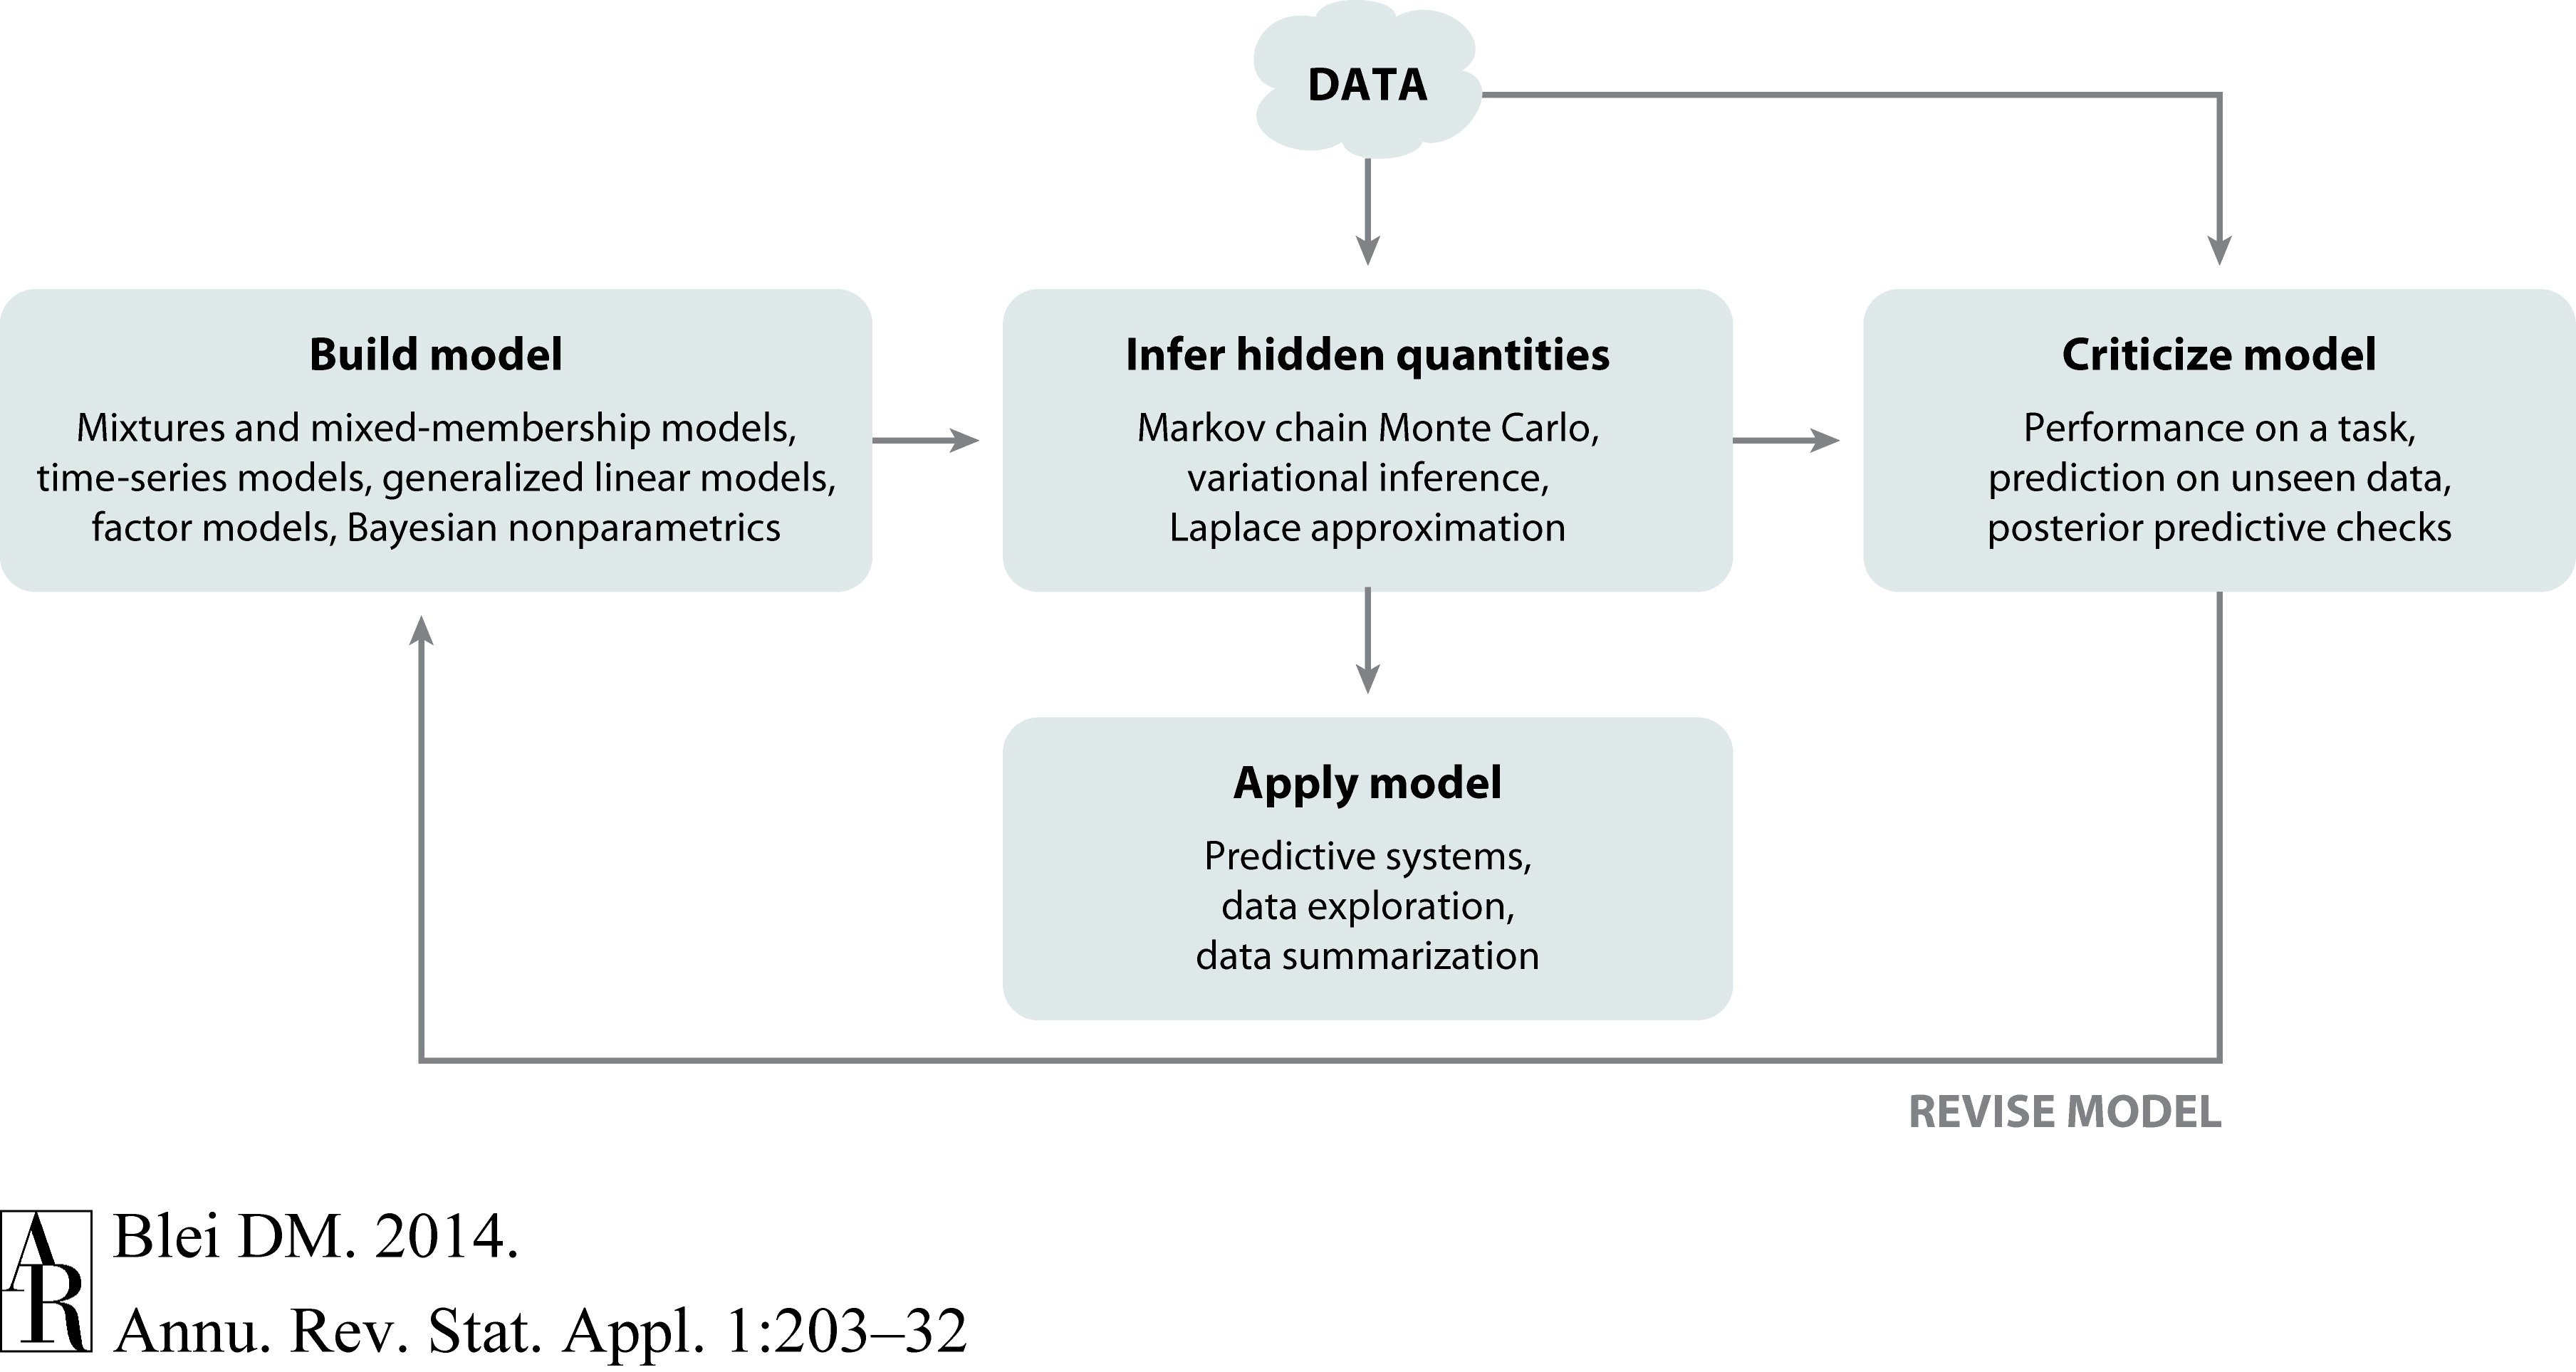
\includegraphics[width=.85\linewidth]{figures/lap1/boxsloop.jpeg}\\
\end{center} 
\begin{flushright}
{\footnotesize Blei, \textit{Ann. Rev. Stat. App.} 2014.}
\end{flushright}
\end{frame}

\begin{frame}{Lap 6: Factor Analysis, Variational Autoencoders, and Variational EM}
Let's walk before we run...
\begin{itemize}
    \item \hyperref[sec:fa]{\textbf{Model:} Factor Analysis}
    \item \hyperref[sec:em]{\textbf{Algorithm:} Expectation Maximization}
\end{itemize}
Next time
\begin{itemize}
    \item \hyperref[sec:vaes]{\textbf{Model:} Nonlinear factor analysis}
    \item \hyperref[sec:vem]{\textbf{Algorithm:} Variational EM}
    \item \hyperref[sec:vaes]{\textbf{Model+Algorithm:} Variational Autoencoders}
\end{itemize}
\end{frame}

\section{Model: Factor Analysis}
\label{sec:fa}

\begin{frame}{The road map}
\end{frame}

\begin{frame}{Factor Analysis}

% \textbf{Idea: } Linear regression with latent (random) covariates. 

% \textbf{Goal \#1: } Learn weights to maximize the marginal likelihood of the observations. 

% \textbf{Goal \#2: } Given weights, infer covariates for each observation.
\end{frame}

\begin{frame}{Notation}
Let,
\begin{itemize}
    \item $\mbx_n \in \reals^D$ denote the $n$-th observation,
    \item $\mbz_n \in \reals^P$ denote the corresponding latent variables,
    \item $\mbw_d \in \reals^{P}$ for $d=1,\ldots,D$ denote the weights each dimension,
    \item $\mbW \in \reals^{D \times P}$ denote the matrix with rows $\mbw_d$.
    \item $\sigma_d^2 \in \reals_+$ for $d=1,\ldots,D$ denote the variance for each dimension, 
    \item $\mbSigma = \diag([\sigma_1^2, \ldots, \sigma_D^2])$ denote the full covariance matrix, amd
    \item $\mbTheta = (\mbW, \mbSigma) = \{\mbw_d, \sigma_d^2\}_{d=1}^D$ denote the set of all parameters.
\end{itemize}
\end{frame}

\begin{frame}{The generative process}
\textbf{Factor analysis} is a ``linear Gaussian'' latent variable model with the following generative process,

To generate $N$ observations $\mbx_1,\ldots, \mbx_N$, each in $\mathbb{R}^D$, 
\begin{enumerate}
    \item Sample model parameters $\{\mbw_d, \sigma_d^2\}_{d=1}^D$ from their prior distribution. 
    \item For each observation $n=1,\ldots,N$,
    \begin{enumerate}[a.]
        \item Sample a \textbf{latent variable} from a multivariate Gaussian prior, $\mbz_n \sim \cN(\mbzero, \mbI)$.
        \item For each dimension $d=1,\ldots,D$
        \begin{enumerate}[i.]
        \item Apply a \textbf{linear transformation} to get the mean $\mbw_d^\top \mbz_n$
        \item Sample the $d$-th coordinate of the \textbf{observation} $x_{n,d} \sim \cN(\mbw_d^\top \mbz_n, \sigma_d^2)$.
        \end{enumerate}
    \end{enumerate}
\end{enumerate}

Note: The last two steps are equivalent to sampling $\mbx_n \sim \cN(\mbW \mbz_n, \mbSigma)$ since $\mbSigma$ is diagonal.
\end{frame}

\begin{frame}{The joint distribution}
The joint probability is,
\begin{align}
    p(\{\mbx_n, \mbz_n\}_{n=1}^N, \mbTheta) 
    &= p(\mbTheta) \prod_{n=1}^N p(\mbx_n \mid \mbz_n, \mbTheta) \; p(\mbz_n \mid \mbTheta) \\
    \label{eq:fa-joint2}
    &= p(\mbTheta) \prod_{n=1}^N \cN(\mbx_n \mid \mbW \mbz_n, \mbSigma) \; \cN(\mbz_n \mid \mbzero, \mbI) \\
    &= p(\mbTheta) \prod_{n=1}^N \prod_{d=1}^D \Big[ \cN(\mbx_n \mid \mbw_d^\top \mbz_n, \sigma_d^2) \big] \; \cN(\mbz_n \mid \mbzero, \mbI) 
\end{align}
We'll place an uninformative prior over the parameters,
\begin{align}
    p(\mbTheta) = p(\{\mbw_d, \sigma_d^2\}_{d=1}^D) 
    \propto \prod_{d=1}^D \sigma_d^{-2}
\end{align}
(Recall from Lap 1 that this is the uninformative limit of a normal inverse chi-squared distribution, $\distInvChiSq(\sigma_d^2 \mid \nu, \tau^2) \, \cN(\mbw_d \mid \mbmu, \sigma_d^2 \mbLambda^{-1})$, with $\nu \to 0$ and $\mbLambda \to 0$.)

% We won't be Bayesian about the parameters. Just give them an improper uniform prior,~$p(\mbTheta) \propto 1$.

% (Note: you could put a matrix normal inverse chi-squared prior on each $(\mbw_d, \sigma_d^2)$; recall Lap 1.)
\end{frame}

\begin{frame}{Warm up: Derive the Gibbs updates}

Suppose we want to sample the posterior distribution, $p(\{\mbw_d, \sigma_d^2\}_{d=1}^D, \{\mbz_n\}_{n=1}^N \mid \{\mbx_n\}_{n=1}^N)$. 

The posterior does not have a simple closed form, but as we learned, we can use MCMC algorithms to produce such samples. 

The Gibbs sampler is one type of MCMC algorithm. It iteratively samples one (or more) variables from their conditional distribution, holding the rest fixed.

For the factor analysis model, this amounts to repeating the following steps \textit{ad infinitum}:
\begin{enumerate}
    \item for $n=1,\ldots,N$, sample $\mbz_n \sim p(\mbz_n \mid \mbx_n, \{\mbw_d, \sigma_d^2\}_{d=1}^D)$
    \item for $d=1,\ldots,D$, sample $\mbw_d, \sigma_d^2 \sim p(\mbw_d, \sigma_d^2 \mid \{\mbx_{n}, \mbz_n\}_{n=1}^N)$
\end{enumerate}
(Note: we used the fact that $\mbz_n$ is conditionally indepedent of $\{\mbx_{n'}, \mbz_{n'}\}_{n'\neq n}$ given the parameters and $\mbw_d, \sigma_d^2$ are conditionally independent of $\{\mbw_{d'}, \sigma_{d'}^2\}_{d'=1}^D$ given the latent variables.)

\end{frame}

\begin{frame}[t]{Warm up: Derive the Gibbs updates II}
\textbf{Exercise: } Derive the conditional distribution $\mbz_n \sim p(\mbz_n \mid \mbx_n, \{\mbw_d, \sigma_d^2\}_{d=1}^D)$. 
\\
\textit{Hint: it's easier to start with Eq.~\ref{eq:fa-joint2} and work with the matrices $\mbW$ and $\mbSigma$.}
\end{frame}

\begin{frame}[t]{Warm up: Derive the Gibbs updates III}
\textbf{Exercise: } Derive the conditional distribution $p(\mbw_d, \sigma_d^2 \mid \{\mbx_{n}, \mbz_n\}_{n=1}^N)$. \\
\textit{Hint: Recall the posterior distribution for Bayesian linear regression model from Lap 1.}
\end{frame}


\begin{frame}{Should we parameters and latent variables the same?}

Gibbs samplings aims for a full posterior distribution over both latent variables and parameters. This is great but perhaps overkill...

In probabilistic machine learning, we often talk about \textit{learning} the parameters and \textit{inferring} the parameters. 

The distinction makes sense when there is more uncertainty about the latent variables~$\mbz_n$, which are informed by a single data point, than about the parameters~$\mbTheta$, which depend on all the data. 

In that case, we might only need a \textit{point estimate} of the parameters and a \textit{posterior} of the latent variables given the data and parameters.
\end{frame}

\begin{frame}{Two goals}
The \textbf{learning goal} is to find the parameters that \textbf{maximize the marginal probability of the data},
\begin{align}
    \mbTheta^\star 
    &= \argmax_{\mbTheta} p(\{\mbx_n\}_{n=1}^N, \mbTheta)\\
    &= \argmax_{\mbTheta} p(\mbTheta) \, \prod_{n=1}^N \int p(\mbx_n \mid \mbz_n, \mbTheta) \, p(\mbz_n \mid \mbTheta) \dif \mbz_n
\end{align}

The \textbf{inference goal} is to find the \textbf{posterior distribution of latent variables},
\begin{align}
    p(\mbz_n \mid \mbx_n, \mbTheta) 
    &= \frac{p(\mbx_n \mid \mbz_n, \mbTheta) \, p(\mbz_n \mid \mbTheta) \, p(\mbTheta)}{p(\mbx_n, \mbTheta)} \\
    &= \frac{p(\mbx_n \mid \mbz_n, \mbTheta) \, p(\mbz_n \mid \mbTheta)}{\int p(\mbx_n \mid \mbz_n, \mbTheta) \, p(\mbz_n \mid \mbTheta)\dif \mbz_n}
\end{align}

Both goals require an integral over $\mbz_n$, and this could potentially be hard!
\end{frame}


\section{Algorithm: EM}
\label{sec:em}


\begin{frame}{Learning via gradient ascent}
Let's start with the learning goal. We could try gradient ascent... 

\begin{align}
    \nabla \log p(\{\mbx_n\}_{n=1}^N, \mbTheta) 
    &= \nabla \log p(\mbTheta) + \sum_{n=1}^N 
    \nabla \log \int p(\mbx_n \mid \mbz_n, \mbTheta) \, p(\mbz_n \mid \mbTheta) \dif \mbz_n \\
    &= \nabla \log p(\mbTheta) + \sum_{n=1}^N 
    \frac{ \int \nabla p(\mbx_n \mid \mbz_n, \mbTheta) \, p(\mbz_n \mid \mbTheta) \dif \mbz_n}{\int p(\mbx_n \mid \mbz_n, \mbTheta) \, p(\mbz_n \mid \mbTheta) \dif \mbz_n }
\end{align}

For conjugate exponential family models, we can get a nice closed form gradient expression, but in general this is tricky.

Moreover, gradient ascent requires choices of a step size, and while that's not so difficult, it is a consideration.

\end{frame}

\begin{frame}[t]{Return of the ELBO}
\textbf{Idea: } Use the ELBO to get a bound on the marginal probability and maximize that instead.
\begin{align}
\log p(\{\mbx_n\}_{n=1}^N, \mbTheta) &= \log p(\{\mbx_n\}_{n=1}^N \mid \mbTheta) + \log p(\mbTheta) \\
&\geq \E_q\left[ \log p(\{\mbx_n, \mbz_n\}_{n=1}^N \mid \mbTheta) - \log q(\{\mbz_n\}_{n=1}^N) \right] + \log p(\mbTheta)\\
&\triangleq \cL(q, \mbTheta)
\end{align}
Here, I've explicitly written the ELBO as a function of both the distribution $q(\{\mbz_n\}_{n=1}^N)$ and the parameters $\mbTheta$.

\end{frame}

\begin{frame}[t]{When is the ELBO tight?}
\textit{Show that the ELBO is maximized when $q(\{\mbz_n\}_{n=1}^N) = p(\{\mbz_n\}_{n=1}^N \mid \{\mbx_n\}_{n=1}^N, \mbTheta)$.}
\end{frame}


\begin{frame}{The Expectation-Maximization (EM) algorithm}

The \textbf{expectation-maximization (EM) algorithm} maximizes this lower bound by iteratively optimizing wrt $q$ and $\mbTheta$. 

\begin{enumerate}
    \item Initialize parameters $\mbTheta$
    \item Repeat until $\mbTheta$ (or the ELBO) converges:
    \begin{enumerate}[a.]
        \item \textbf{E step: } Set
        \begin{align}
            q(\{\mbz_n\}_{n=1}^N) = \argmax_q \cL(q, \mbTheta) = p(\{\mbz_n\}_{n=1}^N \mid \{\mbx_n\}_{n=1}^N, \mbTheta).
        \end{align}
        At this point, the ELBO is tight and $\cL(q, \mbTheta) = p(\{\mbx_n\}_{n=1}^N, \mbTheta)$. Track this quantity!
        \item \textbf{M step: } Set 
        \begin{align}
            \mbTheta &= \argmax_{\mbTheta} \cL(q, \mbTheta) \\
            &= \argmax_{\mbTheta} \E_q[\log p(\{\mbx_n, \mbz_n\}_{n=1}^N \mid \mbTheta)] + \log p(\mbTheta).
        \end{align}
        The optimization in the second step can often be done in closed form. 
    \end{enumerate}
\end{enumerate}
\end{frame}

\begin{frame}{The EM algorithm in pictures}
\begin{center}
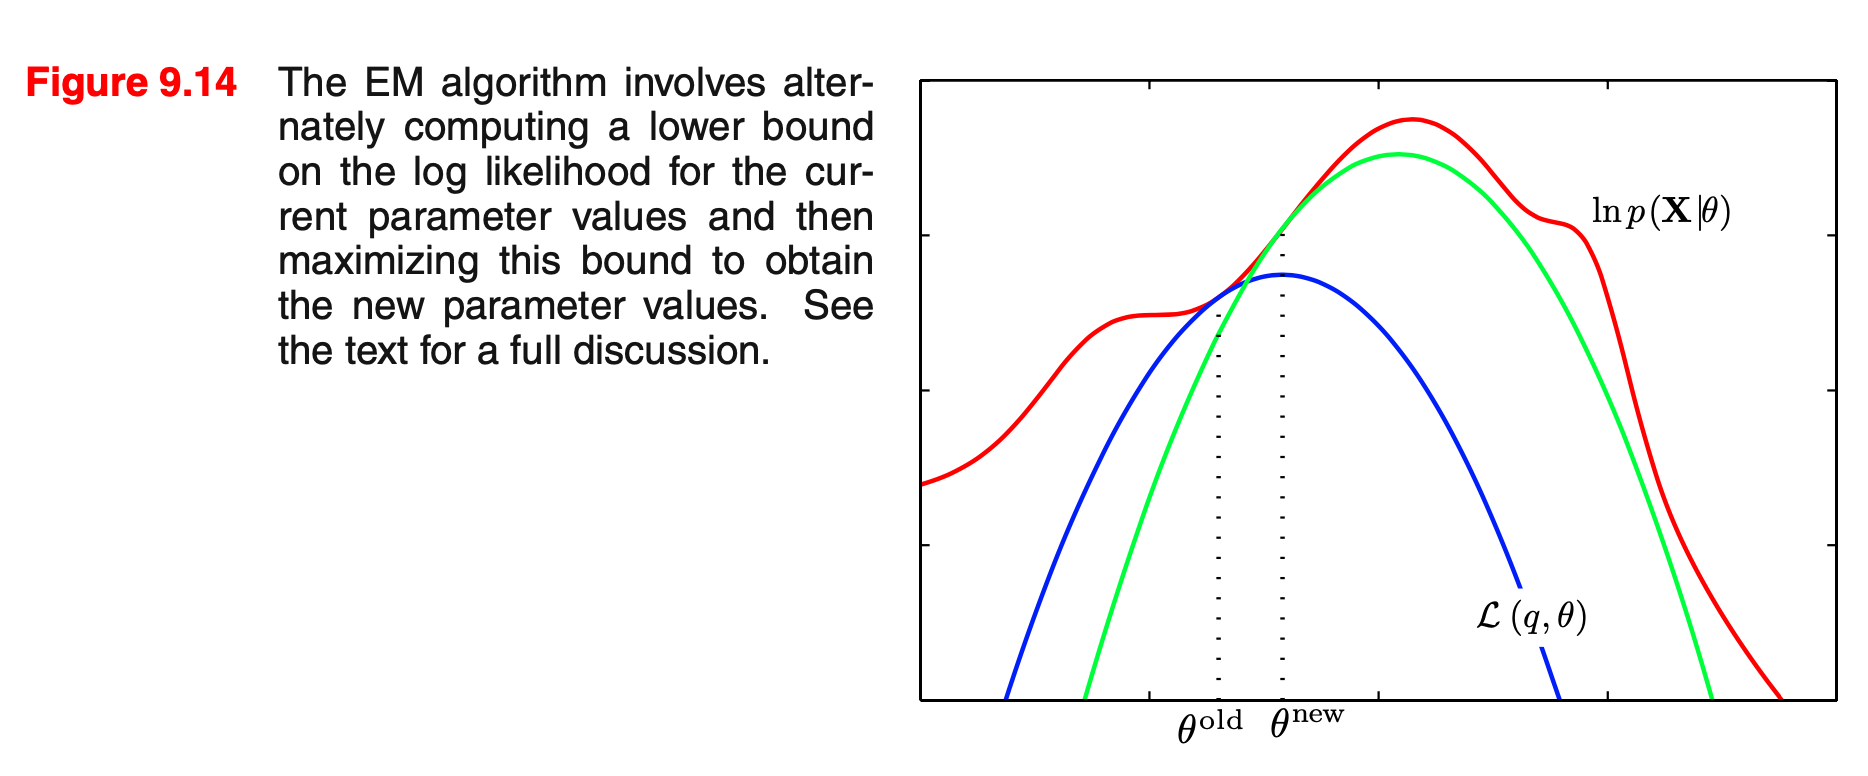
\includegraphics[width=.8\textwidth]{figures/lap6/em.png}    
\end{center}

\hfill From \citet{bishop2006pattern}.

\end{frame}

\begin{frame}{E step for factor analysis}
We've already derived the posterior,
\begin{align}
    p(\{\mbz_n\}_{n=1}^N \mid \{\mbx_n\}_{n=1}^N, \mbTheta)
    &= \prod_{n=1}^N p(\mbz_n \mid \mbx_n, \mbTheta) \\
    &= \prod_{n=1}^N \cN(\mbz_n \mid \mbm_n', \mbC_n') 
\end{align}
where
\begin{align}
    \mbJ_n' &= \mbI + \mbW^\top \mbSigma^{-1} \mbW &
    \mbh_n' &= \mbW^\top \mbSigma^{-1} \mbx_n \\
    \mbC_n' &= \mbJ_n'^{-1} & \mbm_n' &= \mbJ_n'^{-1} \mbh_n'.
\end{align}
\end{frame}

\begin{frame}{M step for factor analysis}

\textbf{Intuition: } Given $\mbz$, this is basically a (Bayesian) linear regression problem.

As a function of $\mbTheta = \{\mbw_d, \sigma_d^2\}_{d=1}^D$,
\begin{align}
    \cL(q, \mbTheta) &= \E_q[\log p(\{\mbx_n, \mbz_n\}_{n=1}^N, \mbTheta)] \\
    &= \E_q \left[\sum_{n=1}^N \log p(\mbx_n \mid \mbz_n, \mbTheta) \right] + \log p(\mbTheta) + c\\
    &= -\frac{1}{2}\sum_{n=1}^N \sum_{d=1}^D \left( \log \sigma_d^2 + \E_{q(\mbz_n)}\left[\frac{1}{\sigma_d^2} (x_{n,d} - \mbw_d^\top \mbz_n)^2 \right]  \right) - \sum_{d=1}^D \log \sigma_d^2 \\\
    &= \sum_{d=1}^D \left[ -\frac{N+2}{2} \log \sigma_d^2  
    - \Big \langle \frac{1}{2 \sigma_d^2}, \sum_{n=1}^N x_{n,d}^2 \Big \rangle
    + \Big \langle \frac{\mbw_d}{\sigma_d^2}, \sum_{n=1}^N \E_q[\mbz_n] x_{n,d} \Big \rangle
    - \Big \langle \frac{\mbw_d \mbw_d^\top}{2\sigma_d^2}, \sum_{n=1}^N \E_q[\mbz_n \mbz_n^\top] \Big \rangle \right] 
    % \\
    % &=
    % \sum_{d=1}^D \left[ \log \distInvChiSq(\sigma_d^2 \mid \nu_d', \tau_d'^2) + \log \cN(\mbw_d \mid \mbmu_d', \sigma_d^2 \mbLambda_d' \right]
\end{align}
We recognize the term in the square brackets as the log of a normal inverse chi-squared distribution, the posterior in a Bayesian linear regression!
\end{frame}

\begin{frame}{M step for factor analysis II}
Recalling Lap 1, we have
\begin{align}
    \cL(q, \mbTheta) &= \E_q[\log p(\{\mbx_n, \mbz_n\}_{n=1}^N, \mbTheta)]
    \sum_{d=1}^D \left[ \log \distInvChiSq(\sigma_d^2 \mid \nu_d', \tau_d'^2) + \log \cN(\mbw_d \mid \mbmu_d', \sigma_d^2 \mbLambda_d') \right]
\end{align}
where
\begin{align}
    \nu_d' &= N &
    \mbLambda_d' &= \sum_{n=1}^N \E_q[\mbz_n \mbz_n^\top] \\
    \mbmu_d' &= \mbLambda_d'^{-1} \sum_{n=1}^N \E_q[\mbz_n] x_{n,d} &
    \tau_d'^2 &= \frac{1}{\nu_d'} \left( \sum_{n=1}^N x_{n,d}^2 - \mbmu_d'^\top  \mbLambda_d' \mbmu_d' \right)
\end{align}
\end{frame}

\begin{frame}{M step for factor analysis III}
The maximum is achieved at the mode of this distribution,
\begin{align}
    \mbw_d &\leftarrow \mbmu_d' = \left( \sum_{n=1}^N \E_q[\mbz_n \mbz_n^\top] \right)^{-1} \left( \sum_{n=1}^N \E_q[\mbz_n] x_{n,d} \right) \\
    \sigma_d^2 &\leftarrow \frac{\nu_d' \tau_d'^2}{\nu_d' + 2}  = \frac{1}{N+2} \left(\sum_{n=1}^N x_{n,d}^2 - \left( \sum_{n=1}^N \E_q[\mbz_n] x_{n,d} \right)^\top \left( \sum_{n=1}^N \E_q[\mbz_n \mbz_n^\top] \right)^{-1} \left( \sum_{n=1}^N \E_q[\mbz_n] x_{n,d} \right) \right)
\end{align}
It's exactly like in Lap 1, except here we have \textbf{expected sufficient statistics} of the latent variables instead of observed covariates.
\end{frame}

\begin{frame}{The big picture}
EM for latent variable models like factor analysis basically iterates between two steps:
\begin{enumerate}
    \item Compute the posterior of the latent variables given the current parameters,
    \item Find the parameters that maximize the expected log joint probability.
\end{enumerate}

For many models (factor analysis, mixture models, etc.), these two steps can be done exactly. 

In practice, EM often converges very quickly, but the objective is non-convex so you might need to try many random initializations!

\end{frame}

\begin{frame}{Questions}
    \begin{itemize}
        \item What if we had $\mbx_{n} \sim \cN(f(\mbz_n, \mbTheta), \mbSigma)$ for some nonlinear function $f$? Where did we use the linearity assumption?
        
        \item What can we do if the posterior needed for the E step is intractable?
        
        \item What if the M step doesn't have a closed form solution?
    \end{itemize}
    
    As we will see, variational autoencoders (VAEs) offer one set of answers to these questions.
\end{frame}


\section{Model: VAEs}
\label{sec:vaes}

\begin{frame}{Lap 6: Factor Analysis, Variational Autoencoders, and Variational EM}
\begin{itemize}
    \item \hyperref[sec:fa]{\textbf{Model:} Factor Analysis}
    \item \hyperref[sec:em]{\textbf{Algorithm:} Expectation Maximization}
    \item \textbf{\hyperref[sec:vaes]{\textbf{Model:} Nonlinear factor analysis}}
    \item \hyperref[sec:vem]{\textbf{Algorithm:} Variational EM}
    \item \hyperref[sec:vaes]{\textbf{Model+Algorithm:} Variational Autoencoders}
\end{itemize}
\end{frame}

\begin{frame}{Nonlinear factor analysis}
The linear Gaussian assumption is a very strong constraint on the factor analysis model.
\begin{itemize}
    \item Essentially, it says the data lie in a \textbf{low-dimensional, linear subspace}.
    \item The assumptions led to tractable EM updates, but is that convenience worth the cost?
    \item What if the data is low-dimensional but on a \textbf{nonlinear manifold}?
\end{itemize}
\end{frame}

\begin{frame}{Nonlinear factor analysis II}
    
\textbf{Nonlinear factor analysis} relaxes the linearity assumption in order to capture nonlinear relationships between latent variables and data"
\begin{align}
\mbz_n &\sim \cN(\mbzero, \mbI) \\
\mbx_n &\sim \cN(f(\mbz_n, \mbtheta), \, \mbSigma) \qquad \text{for } d=1,\ldots,D. 
\end{align}
where $f$ is a function mapping the latent variable $\mbz_n$ to expected value of the observation $\mbx_n$, and it is parameterized by $\mbtheta$.

Here we have allowed for arbitrary covariance $\mbSigma$, but it's common to constrain it to be diagonal, like in regular factor analysis. 

\end{frame}

\begin{frame}{Example}
    
\end{frame}

\begin{frame}[t]{Questions}
\begin{itemize}
    \item How should we parameterize $f$?
    \item How can we handle the E-step in nonlinear factor models?
\end{itemize}
\end{frame}

\begin{frame}{Artificial neural networks as nonlinear function classes for $f$}
We'd like a class of nonlinear functions to map $\mbz_n \to \E[\mbx_n]$. 

We've already seen one such mapping in the context of \textit{generalized} linear models (Lap 2). 

There, a nonlinear \textit{mean function} was applied to the output of a linear function, $\mbw^\top \mbz_n$.

Standard \textbf{artificial neural networks} (ANNs) just stack GLMs one on top of the other. 

Each \textbf{layer} applies a linear function followed by an elementwise nonlinearity. 
\begin{align}
    \E[\mbx_n] &= g(\mbW_L g(\mbW_{L-1} g(\ldots g(\mbW_1 \mbz_n +  \mbb_1) \ldots ) + \mbb_{L-1}) + \mbb_L)
\end{align}
where each $\mbW_\ell \in \reals^{P_\ell \times P_{\ell-1}}$, with $P_L=D$ (the data dimension) and $P_0=P$ (the dimension of $\mbz_n$).  

The set of parameters includes $\mbtheta= \{\mbW_\ell, \mbb_\ell\}_{\ell=1}^L$.

Here, $g$ is an elementwise nonlinearity, like a sigmoid, $g(u) = \tanh(u)$, or rectified linear, $g(u) = \max\{u, 0\}$, function. 
\end{frame}

\section{Algorithm: Variational EM}
\label{sec:vem}

\begin{frame}{Lap 6: Factor Analysis, Variational Autoencoders, and Variational EM}
\begin{itemize}
    \item \hyperref[sec:fa]{\textbf{Model:} Factor Analysis}
    \item \hyperref[sec:em]{\textbf{Algorithm:} Expectation Maximization}
    \item \hyperref[sec:vaes]{\textbf{Model:} Nonlinear factor analysis}
    \item \hyperref[sec:vem]{\textbf{Algorithm: Variational EM}}
    \item \hyperref[sec:vaes]{\textbf{Model+Algorithm:} Variational Autoencoders}
\end{itemize}
\end{frame}


\begin{frame}{The Variational Expectation-Maximization (vEM) algorithm}

The \textbf{variational} expectation-maximization (vEM) algorithm maximizes the lower bound by iteratively optimizing wrt $q$ and $\mbTheta$, \textbf{subject to the constraint that $q \in \cQ$.}

\begin{enumerate}
    \item Initialize parameters $\mbTheta$
    \item Repeat until $\mbTheta$ (or the ELBO) converges:
    \begin{enumerate}[a.]
        \item \textbf{E step: } Set
        \begin{align}
            q(\{\mbz_n\}_{n=1}^N; \mblambda) = \argmax_{q \in \cQ} \cL(q, \mbTheta) = \argmin_{q \in \cQ} \KL{q(\{\mbz_n\}_{n=1}^N; \mblambda)}{p(\{\mbz_n\}_{n=1}^N \mid \{\mbx_n\}_{n=1}^N, \mbTheta)}
        \end{align}
        \item \textbf{M step: } Set 
        \begin{align}
            \mbTheta &= \argmax_{\mbTheta} \cL(q, \mbTheta) \\
            &= \argmax_{\mbTheta} \E_q[\log p(\{\mbx_n, \mbz_n\}_{n=1}^N \mid \mbTheta)] + \log p(\mbTheta).
        \end{align}
    \end{enumerate}
\end{enumerate}
\textbf{Question:} is the ELBO tight after the E-step? Will $\mbTheta$ converge to $\argmax_{\mbTheta} p(\{\mbx_n\}_{n=1}^N, \mbTheta)$?
\end{frame}

\begin{frame}{The variational E-step for nonlinear factor analysis}
For nonlinear factor analysis, we know the true posterior factors over data points since,
\begin{align}
    p(\{\mbz_n\}_{n=1}^N \mid \{\mbx_n\}_{n=1}^N, \mbTheta)
    &\propto \prod_{n=1}^N \cN(\mbz_n \mid \mbzero, \mbI) \, \cN(\mbx_n \mid f(\mbz_n, \mbtheta), \mbSigma) \\
    &= \prod_{n=1}^N p(\mbz_n \mid \mbx_n, \mbTheta),
\end{align}
where $\mbTheta = (\mbtheta, \mbSigma)$.

We'll assume the variational posterior factors in the same way,  $q(\{\mbz_n\}_{n=1}^N; \mblambda) = \prod_{n=1}^N q(\mbz_n; \mblambda_n)$.

How can we solve for the optimal factors though?
\begin{align}
    q(\mbz_n; \mblambda_n) 
    % = \argmax_{q \in \cQ} \cL(q, \mbTheta) 
    = \argmin_{q \in \cQ} \KL{q(\mbz_n; \mblambda_n)}{p(\mbz_n \mid \mbx_n, \mbTheta)}
\end{align}
Unfortunately the posterior $p(\mbz_n \mid \mbx_n, \mbTheta)$ is no longer a simple closed-form Gaussian.

\end{frame}

\begin{frame}{Stochastic gradient descent on the KL divergence}
Even though the true posterior is not a Gaussian, let's approximate it with one.  That is, assume,
\begin{align}
    q(\mbz_n ; \mblambda_n) &= \cN(\mbz_n; \mbm_n, \mbC_n)
\end{align}
where $\mblambda_n = (\mbm_n, \mbC_n)$.

Then,
\begin{align}
    &\KL{q(\mbz_n; \mblambda_n)}{p(\mbz_n \mid \mbx_n, \mbTheta)}
    = \E_{q(\mbz_n)}\left[\log q(\mbz_n; \mblambda_n) - \log p(\mbz_n \mid \mbx_n, \mbTheta) \right] \\
    \label{eq:kl}
    &\qquad = \KL{\cN(\mbz_n; \mbm_n, \mbC_n)}{\cN(\mbz_n \mid \mbzero, \mbI)} - \E_{q(\mbz_n; \mblambda_n)} \left[\log p(\mbx_n \mid f(\mbz_n, \mbtheta), \mbSigma) \right]  + c
\end{align}

The first term can be computed in closed form---it's the KL divergence between two Gaussians. 

The second term is harder...
\end{frame}

\begin{frame}{The ``reparameterization trick''}
Note that we can \textbf{reparameterize} the variational posterior as 
\begin{align}
    \mbz_n &\sim \cN(\mbm_n, \mbC_n) &\iff & &
    \mbz_n &= \mbm_n + \mbC_n^{1/2} \mbepsilon_n \\
    & & & & \mbepsilon_n &\sim \cN(\mbzero, \mbI) 
\end{align}
We can use the \textbf{law of the unconscious statistician} to rewrite the expectation in eq.~\ref{eq:kl} as,
\begin{align}
    \E_{q(\mbz_n; \mblambda_n)} \left[\log p(\mbx_n \mid f(\mbz_n, \mbtheta), \mbSigma) \right]
    &= \E_{\mbepsilon_n \sim \cN(\mbzero, \mbI)} \left[\log p(\mbx_n \mid f(\mbm_n + \mbC_n^{1/2} \mbepsilon_n, \, \mbtheta), \mbSigma) \right]
\end{align}
From this representation, we can rewrite the gradient of the KL divergence as,
\begin{multline}
    \nabla_{\mblambda_n} \KL{q(\mbz_n; \mblambda_n)}{p(\mbz_n \mid \mbx_n, \mbTheta)} 
    = 
    \nabla_{\mblambda_n} \KL{\cN(\mbz_n; \mbm_n, \mbC_n)}{\cN(\mbz_n \mid \mbzero, \mbI)} \\
    - \E_{\mbepsilon_n \sim \cN(\mbzero, \mbI)} \left[\nabla_{\mblambda_n} \log p(\mbx_n \mid f(\mbm_n + \mbC_n^{1/2} \mbepsilon_n, \, \mbtheta), \mbSigma) \right]
\end{multline}
and \textbf{use Monte Carlo to obtain an unbiased estimate of the final expectation.}
\end{frame}

\begin{frame}{The variational M-step for nonlinear factor analysis}
The parameters $\mbTheta$ present the same problem: there's no closed form solution so we need to resort to gradient ascent on the ELBO. 

It's slightly easier since $q$ does not depend on $\mbTheta$, allowing us to bring the gradient inside the expectation,
\begin{align}
    \nabla_{\mbTheta} \cL(q, \mbTheta) &= 
    \nabla_{\mbTheta} \E_q \left[ \log p(\{\mbx_n, \mbz_n\}_{n=1}^N \mid \mbTheta) \right] + \nabla_{\mbTheta} \log p(\mbTheta) \\
    &=
    \label{eq:vem_mgrad}
    \sum_{n=1}^N \E_{q(\mbz_n; \mblambda_n)} \left[ \nabla_{\mbTheta} \log \cN(\mbx_n \mid f(\mbz_n, \mbTheta), \mbSigma) \right] + \nabla_{\mbTheta} \log p(\mbTheta)
\end{align}
Again, we can obtain an unbiased Monte Carlo estimate by sampling $q(\mbz_n; \mblambda_n)$.

What about $\mbSigma$? You can learn the observation covariance matrix via gradient descent, just like on $\mbTheta$, but it's common to treat this as a hyperparameter and fix it to $\mbSigma = \sigma^2 \mbI$ for some small-ish $\sigma^2$. 

Then $\sigma^2$ effectively reweights the expected log likelihood and the KL to the prior in the ELBO.
\end{frame}

\begin{frame}{Working with mini-batches of data}
Note that the ELBO involves a sum over data points,
\begin{align}
    \cL(q, \mbTheta) &= \E_q [\log p(\{\mbx_n, \mbz_n\}_{n=1}^N \mid \mbTheta) - \log q(\{\mbz_n\}_{n=1}^N; \mblambda] + \log p(\mbTheta) \\
    &= \E_{q(\{\mbz_n\}_{n=1}^N; \mblambda)} \left[\sum_{n=1}^N \log p(\mbx_n \mid \mbz_n, \mbTheta) + \log p(\mbz_n) - \log q(\mbz_n; \mblambda_n) \right] + \log p(\mbTheta)
    \\
    &= \sum_{n=1}^N \Big(\underbrace{\E_{q(\mbz_n; \mblambda_n)}[\log p(\mbx_n \mid \mbz_n)] - \KL{q(\mbz_n; \mblambda_n)}{p(\mbz_n)}}_{\text{``local ELBO'' } \cL_n(\mblambda_n, \mbTheta)} \Big) + \log p(\mbTheta)
\end{align}

We can view the sum as an ``expectation'' over data indices,
\begin{align}
    \sum_{n=1}^N \cL_n(\lambda_n, \mbTheta) &= N \, \E_{n \sim \distUniform(\{1,\ldots,N\})}[\cL_n(\lambda_n, \mbTheta)],
\end{align}
and we can use Monte Carlo to approximate the expectation and its gradient with respect to $\mbTheta$.
    
\end{frame}

\begin{frame}{Lap 6: Factor Analysis, Variational Autoencoders, and Variational EM}
\begin{itemize}
    \item \hyperref[sec:fa]{\textbf{Model:} Factor Analysis}
    \item \hyperref[sec:em]{\textbf{Algorithm:} Expectation Maximization}
    \item \hyperref[sec:vaes]{\textbf{Model:} Nonlinear factor analysis}
    \item \hyperref[sec:vem]{\textbf{Algorithm:} Variational EM}
    \item \hyperref[sec:vaes]{\textbf{Model+Algorithm: Variational Autoencoders}}
\end{itemize}
\end{frame}

\begin{frame}{Variational Autoencoders (VAEs)}
VAEs are essentially nonlinear factor analysis models trained with variational EM, but they introduce \textbf{one key idea}.

Note that vEM involves a costly E-step to find the variational parameters $\mblambda_n$ for each data point. This could involve many steps of gradient descent inside just the E-step!

With a finite computational budget, we might be better off doing more gradient steps on $\mbTheta$ and fewer on the local variational parameters.

Note that the optimal variational parameters are just a function of the data point and the model parameters,
\begin{align}
    \mblambda_n &= \argmin \KL{q(\mbz_n; \mblambda_n)}{p(\mbz_n \mid \mbx_n, \mbTheta)} 
    \triangleq g^\star(\mbx_n, \mbTheta).
\end{align}
for some implicit and generally nonlinear function $g^\star$.
\end{frame}

\begin{frame}{Inference networks}
VAEs learn an approximation to $g^\star(\mbx_n, \mbTheta)$ with an \textbf{inference network} (also called a \textbf{recognition network}).

The inference network is (yet another) neural network that takes in a data point $\mbx_n$ and outputs variational parameters $\mbz_n$,
\begin{align}
    \mblambda_n & \approx g(\mbx_n, \mbphi),
\end{align}
where $\mbphi$ are the weights of the network.
    
The advantage is that the inference network is very fast; in the E-step, we simply need to pass a data point through the network to obtain the variational parameters.

The disadvantage is the output will not minimize the KL divergence. However, in practice we might tolerate a worse variational posterior and a weaker lower bound if it buys us more updates of~$\mbTheta$.

\end{frame}

\begin{frame}{Amortization and approximation gaps}
    
\citet{cremer2018inference} consider the relative  effects of the \textbf{amortization gap} and the \textbf{approximation gap} on variational EM.

\begin{center}
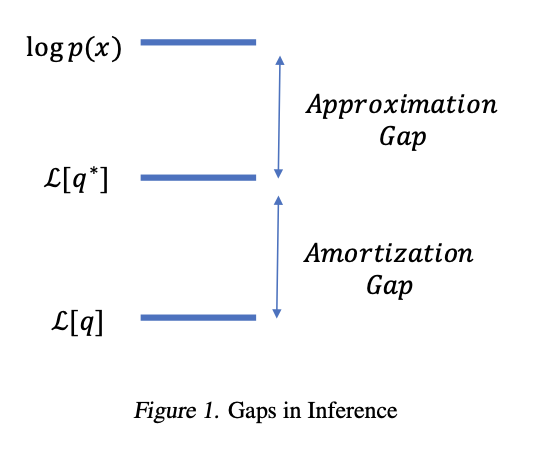
\includegraphics[width=.4\textwidth]{figures/lap6/gaps.png}
\end{center}

\textbf{Question: } How, if at all, does the generative model $p(\mbx_n \mid \mbz_n, \mbTheta)$ affect these gaps? 
\end{frame}

\begin{frame}{VAEs from an autoencoder perspective}
\begin{figure}
    \centering
    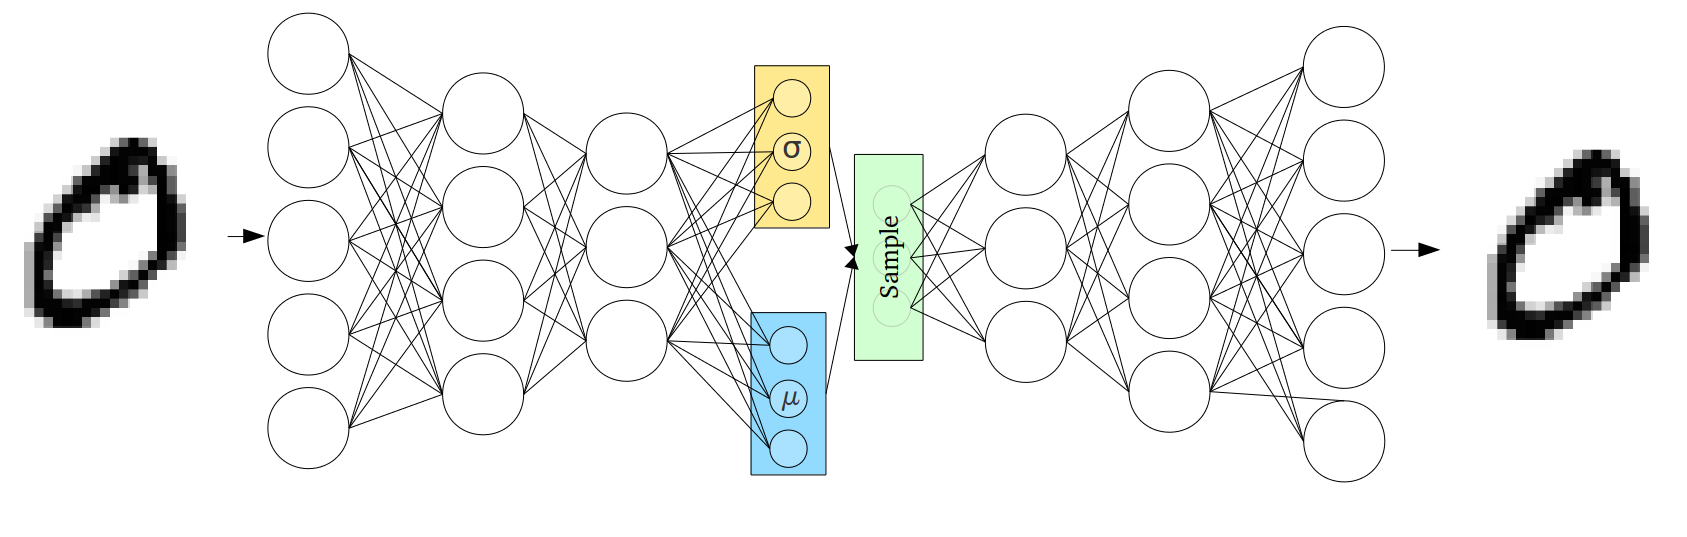
\includegraphics[width=.9\textwidth]{figures/lap6/vae.png}
    \label{fig:vae}
\end{figure}

\footnotesize From \url{https://towardsdatascience.com/intuitively-understanding-variational-autoencoders-1bfe67eb5daf}
\end{frame}

\begin{frame}[t]{Linear VAEs}
\textbf{Question: } What does the optimal encoder network look like for linear factor analysis?
    
\end{frame}

\begin{frame}[t,allowframebreaks]
        \frametitle{References}
        \bibliographystyle{unsrtnat}
        \bibliography{refs.bib}
\end{frame}

\end{document}